\section{Bayesian Statistics}

\subsection{Recommended References}
\begin{frame}{Bayesian Statistics - Recommended References}
	\begin{vfilleditems}
		\item \textcite{gelman2013bayesian} - Chapter 1: Probability and inference
		\item \textcite{mcelreath2020statistical} - Chapter 1: The Golem of Prague
		\item \textcite{gelman2020regression} - Chapter 3: Some basic methods in mathematics and probability
		\item \textcite{khanBayesianLearningRule2021}
		\item \textbf{Probability}:
		\begin{vfilleditems}
			\item A great textbook - \textcite{bertsekasIntroductionProbability2nd2008}
			\item Also a great textbook (skip the frequentist part)- \textcite{dekkingModernIntroductionProbability2010}
			\item Bayesian point-of-view and also a philosophical approach- \textcite{jaynesProbabilityTheoryLogic2003}
			\item Bayesian point-of-view with a simple and playful approach - \textcite{kurtBayesianStatisticsFun2019}
			\item Philosophical approach not so focused on mathematical rigor - \textcite{diaconisTenGreatIdeas2019}
		\end{vfilleditems}
	\end{vfilleditems}
\end{frame}

\subsection{What is Bayesian Statistics?}
\begin{frame}{What is Bayesian Statistics?}
	Bayesian statistics is a \textbf{data analysis approach based on Bayes' theorem}
	where available knowledge about the parameters of a statistical model
	is updated with the information of observed data.
	\parencite{gelman2013bayesian}.
	Previous knowledge is expressed as a \textbf{prior} distribution
	and combined with the observed data in the form of a \textbf{likelihood} function
	to generate a \textbf{posterior} distribution.
	The posterior can also be used to make predictions about future events.
\end{frame}

\subsubsection{What changes from Frequentist Statistics?}
\begin{frame}{What changes from Frequentist Statistics?}
	\begin{vfilleditems}
		\item \textbf{Flexibility} - probabilistic building blocks to
		construct a model\footnote{like LEGO}:
		\begin{vfilleditems}
			\item Probabilistic conjectures about parameters:
			\begin{vfilleditems}
				\item Prior
				\item Likelihood
			\end{vfilleditems}
		\end{vfilleditems}
		\item Better \textbf{uncertainty} treatment:
		\begin{vfilleditems}
			\item Coherence
			\item Propagation
			\item We don't use \textit{"if we sampled infinite times
				from a population that we do not observe..."}
		\end{vfilleditems}
		\item No \textbf{$p$-values}:
		\begin{vfilleditems}
			\item All statistical intuitions makes \textbf{sense}
			\item 95\% certainty that $\theta$'s parameter value is
			between $x$ and $y$
			\item Almost \textbf{impossible} to perform $p$-hacking
		\end{vfilleditems}
	\end{vfilleditems}
\end{frame}

\begin{frame}{A little bit more formal}
	\begin{vfilleditems}
		\item Bayesian Statistics uses probabilistic statements:
		\begin{vfilleditems}
			\item one or more parameters $\theta$
			\item unobserved data $\tilde{y}$
		\end{vfilleditems}
		\item These statements are conditioned on the observerd values of $y$:
		\begin{vfilleditems}
			\item $P(\theta \mid y)$
			\item $P(\tilde{y} \mid y)$
		\end{vfilleditems}
		\item We also, implicitly, conditioned on the observed data from
		any covariate $x$
	\end{vfilleditems}
\end{frame}

\begin{frame}{Definition of Bayesian Statistics}
	\begin{defn}[Bayesian Statistics]
		The use of Bayes theorem as the procedure to \textbf{estimate
			parameters of interest $\theta$ or unobserved data $\tilde{y}$}.
		\parencite{gelman2013bayesian}
	\end{defn}
\end{frame}

\subsection{Tools}
\begin{frame}{Tools}
	\centering
	\textit{``A man and his tools make a man and his trade''}

	\vspace{2ex}

	Vita Sackville-West
\end{frame}

\begin{frame}{Tools}
	\begin{vfilleditems}
		\item \LARGE  \href{https://mc-stan.org}{\texttt{Stan}} (BSD-3 License)
		\item \LARGE  \href{https://turing.ml}{\texttt{Turing.jl}} (MIT License)
		\item \href{https://www.pymc.io/}{\texttt{PyMC}} (Apache License)
		\item \small \href{https://mcmc-jags.sourceforge.io/}{\texttt{JAGS}} (GPL License)
		\item \footnotesize \href{https://www.mrc-bsu.cam.ac.uk/software/bugs/}{\texttt{BUGS}} (GPL License)
	\end{vfilleditems}
\end{frame}

\subsubsection{Stan}
\begin{frame}{\texttt{Stan}\footnote{\textcite{carpenterStanProbabilisticProgramming2017}}}
	\begin{columns}
		\begin{column}{0.8\textwidth}
			\begin{vfilleditems}
				\small
				\item High-performance platform for statistical
				modeling and  statistical computation
				\item Financial support from
				\href{https://numfocus.org/}{NUMFocus}:
				\begin{vfilleditems}
					\footnotesize
					\item AWS Amazon
					\item Bloomberg
					\item Microsoft
					\item IBM
					\item RStudio
					\item Facebook
					\item NVIDIA
					\item Netflix
				\end{vfilleditems}
				\small
				\item Open-source language, similar to \texttt{C++}
				\item Markov Chain Monte Carlo (MCMC) parallel sampler
			\end{vfilleditems}
		\end{column}
		\begin{column}{0.2\textwidth}
			\centering
			
\includegraphics[width=0.9\textwidth]{stan.png}
		\end{column}
	\end{columns}
\end{frame}

\begin{frame}[fragile]{\texttt{Stan} Code Example}
	\begin{lstlisting}[basicstyle=\footnotesize, language=Stan]
        data {
          int<lower=0> N;
          vector[N] x1;
          vector[N] x2;
          vector[N] y;
        }
        parameters {
          real alpha;
          real beta1;
          real beta2;
          real<lower=0> sigma;
        }
        model {
          alpha ~ normal(0, 20);
          beta1 ~ normal(0, 2);
          beta2 ~ normal(0, 2);
          sigma ~ cauchy(0, 2.5);
          y ~ normal(alpha + beta1 * x1 + beta2 * x2, sigma);
        }
    \end{lstlisting}
\end{frame}

\subsubsection{Turing.jl}
\begin{frame}{\texttt{Turing.jl}\footnote{\textcite{geTuringLanguageFlexible2018}}}
	\begin{columns}
		\begin{column}{0.8\textwidth}
			\begin{vfilleditems}
				\small
				\item Ecosystem of Julia packages for Bayesian
				Inference using probabilistic programming
				\item \href{https://www.julialang.org}{Julia} is a fast
				dynamic-typed language that just-in-time (JIT)
				compiles into native code using LLVM:
				\href{https://www.nature.com/articles/d41586-019-02310-3}{``runs like C but reads like Python''};
				meaning that is \textit{blazing} fast, easy to prototype and read/write code
				\item Julia has Financial support from
				\href{https://numfocus.org/}{NUMFocus}
				\item Composability with other Julia packages
				\item Several other options of Markov Chain Monte Carlo (MCMC) samplers
			\end{vfilleditems}
		\end{column}
		\begin{column}{0.2\textwidth}
			\centering
			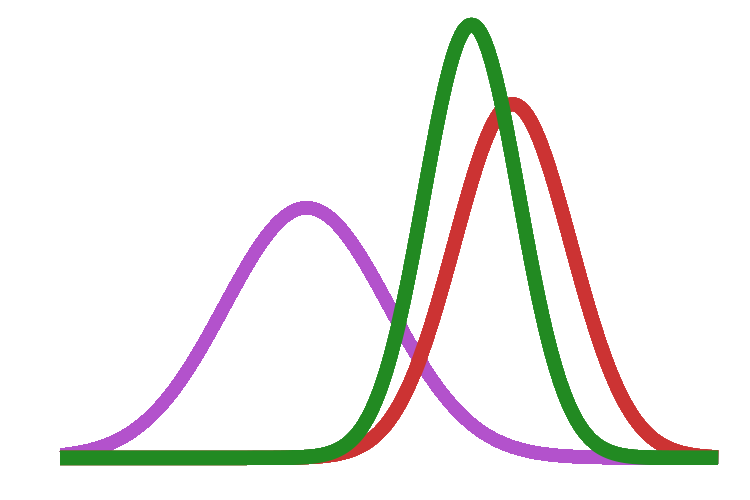
\includegraphics[width=0.9\textwidth]{turing.png}
		\end{column}
	\end{columns}
\end{frame}

\begin{frame}{\texttt{Turing.jl} Ecosystem}
	We have several Julia packages under \texttt{Turing.jl}'s GitHub
	organization \href{https://github.com/TuringLang}{TuringLang},
	but I will focus on 6 of those:

	\begin{vfilleditems}
		\small
		\item \href{https://github.com/TuringLang/Turing.jl}{\texttt{Turing.jl}}:
		main package that we use to \textbf{interface with all
			the Turing ecosystem} of packages and the backbone of
		everything
		\item \href{https://github.com/TuringLang/MCMCChains.jl}{\texttt{MCMCChains.jl}}:
		interface to \textbf{summarizing MCMC simulations} and
		has several utility functions for \textbf{diagnostics}
		and \textbf{visualizations}
		\item \href{https://github.com/TuringLang/DynamicPPL.jl}{\texttt{DynamicPPL.jl}}:
		specifies a domain-specific language for \texttt{Turing.jl},
		entirely written in Julia, and it is modular
		\item \href{https://github.com/TuringLang/AdvancedHMC.jl}{\texttt{AdvancedHMC.jl}}:
		modular and efficient implementation of advanced
		Hamiltonian Monte Carlo (HMC) algorithms
		\item \href{https://github.com/TuringLang/DistributionsAD.jl}{\texttt{DistributionsAD.jl}}:
		defines the necessary functions to enable automatic
		differentiation (AD) of the log PDF functions from
		\href{https://github.com/JuliaStats/Distributions.jl}{\texttt{Distributions.jl}}
		\item \href{https://github.com/TuringLang/Bijectors.jl}{\texttt{Bijectors.jl}}:
		implements a set of functions for transforming constrained
		random variables (\textit{e.g.} simplexes, intervals)
		to Euclidean space
	\end{vfilleditems}
\end{frame}

\begin{frame}[fragile]{\texttt{Turing.jl}\footnote{
			I believe in Julia's potential and wrote a whole set of
			\href{https://storopoli.io/Bayesian-Julia}{
				Bayesian Statistics tutorials using Julia and
				\texttt{Turing.jl}} \parencite{storopoli2021bayesianjulia}}
		Code Example}
	\begin{lstlisting}[basicstyle=\small, language=Matlab, escapeinside=\{\}]
        @model linreg({$x_1$}, {$x_2$}, y) = begin
            {$\alpha$} ~ Normal(0, 20)
            {$\beta_1$} ~ Normal(0, 2)
            {$\beta_2$} ~ Normal(0, 2)
            {$\sigma$} ~ truncated(Cauchy(0, 2.5); lower=0)

            y .~ Normal({$\alpha$} .+ {$\beta_1$} * {$x_1$} + {$\beta_2$} * {$x_2$}, {$\sigma$})
        end
    \end{lstlisting}
\end{frame}

\begin{frame}{\texttt{Stan} and \texttt{Julia} mentioned in Billions\footnote{
			If you cannot watch the video \href{https://github.com/storopoli/Bayesian-Statistics/blob/main/images/stan_billions_subtitled.mp4?raw=true}{click here}
			to see it in your browser.} (Season 3 Episode 9)}
	\centering
	\includemedia[
		width=\linewidth,
		height=0.3\linewidth,
		addresource=stan_billions_subtitled.mp4,
		transparent,
		activate=pageopen,
		passcontext,  %show VPlayer's right-click menu
		flashvars={
				source=stan_billions_subtitled.mp4
				&loop=true
				&scaleMode=stretch
			}
	]{\texttt{Stan} and Julia mentioned in Billions}{http://mirrors.ctan.org/macros/latex/contrib/media9/players/VPlayer.swf}
\end{frame}

\subsubsection{PyMC}
\begin{frame}{\texttt{PyMC}\footnote{\textcite{pymc3}}}
	\begin{columns}
		\begin{column}{0.8\textwidth}
			\begin{vfilleditems}
				\small
				\item Python package for Bayesian statistics
				with a Markov Chain Monte Carlo sampler
				\item Financial support from \href{https://numfocus.org/}{NUMFocus}
				\item Backend was based on \texttt{Theano}
				\item \texttt{Theano} \textbf{died}, but \texttt{PyMC} developers create a fork
				named \texttt{Aesara}
				\item We have no idea what will be the backend in
				the future.
				\texttt{PyMC} developers are still experimenting with other
				backends: \texttt{TensorFlow Probability}, \texttt{NumPyro}
				and so on ...
			\end{vfilleditems}
		\end{column}
		\begin{column}{0.2\textwidth}
			\centering
			
\includegraphics[width=0.9\textwidth]{pymc.png}
		\end{column}
	\end{columns}
\end{frame}

\begin{frame}[fragile]{\texttt{PyMC} Code Example}
	\begin{lstlisting}[basicstyle=\small, language=Python]
    with pm.Model() as model:
        alpha = pm.Normal("Intercept", mu=0, sigma=20)
        beta_1 = pm.Normal("beta_1", mu=0, sigma=2)
        beta_2 = pm.Normal("beta_2", mu=0, sigma=2)
        sigma = pm.HalfCauchy("sigma", beta=2.5)

        likelihood = pm.Normal("y",
                     mu=alpha + beta_1 * x1 + beta_2 * x2,
                     sigma=sigma, observed=y)
\end{lstlisting}
\end{frame}

\subsection{Probability}
\begin{frame}{PROBABILITY DOES NOT EXIST!\footnote{\textcite{definettiTheoryProbability1974}}}
	\begin{columns}
		\begin{column}{0.8\textwidth}
			\begin{vfilleditems}
				\item Yes, probability does not exist ...
				\item Or even better, probability as a physical quantity,
				objective chance, \textbf{does NOT exist}
				\item if we disregard objetive chance \textit{nothing is lost}
				\item The math of inductive rationality remains
				\textbf{exactly the same}
			\end{vfilleditems}
		\end{column}
		\begin{column}{0.2\textwidth}
			\centering
			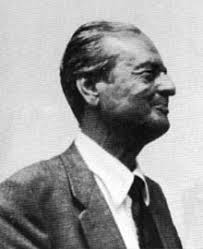
\includegraphics[width=0.9\columnwidth]{finetti.jpg}
		\end{column}
	\end{columns}
\end{frame}

\begin{frame}{PROBABILITY DOES NOT EXIST!\footnote{\textcite{definettiTheoryProbability1974}}}
	\begin{columns}
		\begin{column}{0.6\textwidth}
			\begin{vfilleditems}
				\small
				\item Consider flipping a biased coin
				\item The trials are considered independent and, as a result,
				have an important property: \textbf{the order does not matter}
				\item The frequency is considered a \textbf{sufficient statistic}
				\item Saying that order does not matter or saying that the only thing that
				matters is frequency are two ways of saying the same thing
				\item We say that the probability is \textbf{invariant under permutations}
			\end{vfilleditems}
		\end{column}
		\begin{column}{0.4\textwidth}
			\begin{tikzpicture}[
					scale=0.55,
					transform shape, thick,
					every node/.style = {draw, circle, minimum size = 10mm},
					grow = down,  % alignment of characters
					level 1/.style = {sibling distance=3cm},
					level 2/.style = {sibling distance=1.5cm},
					level 3/.style = {sibling distance=3cm},
					level distance = 3cm,
					head/.style = {fill = orange!90!blue,
							label = center:\textsf{\Large H}},
					tail/.style = {fill = blue!70!yellow, text = black,
							label = center:\textsf{\Large T}}
				]
				\node[shape = circle split, draw, line width = 1pt,
					minimum size = 10mm, inner sep = 0mm, font = \sffamily\large,
					rotate=30] (Start)
				{ \rotatebox{-30}{H} \nodepart{lower} \rotatebox{-30}{T}}
				child {   node [head] (A) {}
						child { node [head] (B) {}}
						child { node [tail] (C) {}}
					}
				child {   node [tail] (D) {}
						child { node [head] (E) {}}
						child { node [tail] (F) {}}
					};

				% Filling the root (Start)
				\begin{scope}[on background layer, rotate=30]
					\fill[head] (Start.base) ([xshift = 0mm]Start.east) arc (0:180:5mm)
					-- cycle;
					\fill[tail] (Start.base) ([xshift = 0pt]Start.west) arc (180:360:5mm)
					-- cycle;
				\end{scope}

				% Labels
				\begin{scope}[nodes = {draw = none}]
					\path (Start) -- (A) node [near start, left]  {$0.5$};
					\path (A)     -- (B) node [near start, left]  {$0.5$};
					\path (A)     -- (C) node [near start, right] {$0.5$};
					\path (Start) -- (D) node [near start, right] {$0.5$};
					\path (D)     -- (E) node [near start, left]  {$0.5$};
					\path (D)     -- (F) node [near start, right] {$0.5$};
					\begin{scope}[nodes = {below = 11pt}]
						\node at (B) {$0.25$};
						\node at (C) {$0.25$};
						\node at (E) {$0.25$};
						\node at (F) {$0.25$};
					\end{scope}
				\end{scope}
			\end{tikzpicture}
		\end{column}
	\end{columns}
\end{frame}

\begin{frame}{Probability Interpretations}
	\begin{vfilleditems}
		\item \textbf{Objective} - frequency in the long run for an event:
		\begin{vfilleditems}
			\item $P(\text{rain}) = \frac{\text{days that rained}}{\text{total days}}$
			\item $P(\text{me being elected president}) = 0$ (never occurred)
		\end{vfilleditems}
		\item \textbf{Subjective} - degrees of belief in an event:
		\begin{vfilleditems}
			\item $P(\text{rain}) = \text{degree of belief that will rain}$
			\item $P(\text{me being elected president}) = 10^{-10}$ (highly unlikely)
		\end{vfilleditems}
	\end{vfilleditems}
\end{frame}

\subsubsection{What is Probability?}
\begin{frame}{What is Probability?}
	\begin{defn}[Probability]
		We define $A$ is an event and $P(A)$ the probability of event $A$.
		$P(A)$ has to be between $0$ and $1$, where higher values defines
		higher probability of $A$ happening.
		$$\begin{aligned}
				P(A)   & \in \mathbb{R} \\
				P(A)   & \in [0,1]      \\
				0 \leq & P(A) \leq 1
			\end{aligned}$$
	\end{defn}
\end{frame}

\begin{frame}{Probability Axioms\footnote{\textcite{kolmogorovFoundationsTheoryProbability1933}}}
	\begin{columns}
		\begin{column}{0.8\textwidth}
			\begin{vfilleditems}
				\item \textbf{Non-negativity}: For every $A$:
				$$P(A) \geq 0$$
				\item \textbf{Additivity}: For evey two \textit{mutually exclusive}
				$A$ and $B$:
				$$P(A) = 1 - P(B) \text{ and } P(B) = 1 - P(A)$$
				\item \textbf{Normalization}: The probability of all possible
				events $A_1, A_2, \dots$ must sum up to $1$:
				$$\sum_{n \in \mathbb{N}} A_n = 1$$
			\end{vfilleditems}
		\end{column}
		\begin{column}{0.2\textwidth}
			\centering
			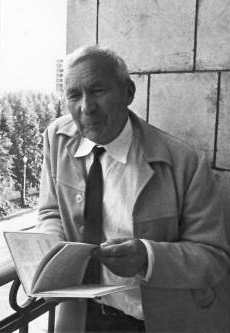
\includegraphics[width=0.9\columnwidth]{kolmogorov.jpg}
		\end{column}
	\end{columns}
\end{frame}

\begin{frame}{Sample Space}
	\begin{vfilleditems}
		\item Discrete $$\Theta = \left\{1, 2, \ldots \right\}$$
		\item Continuous $$\Theta \in \left(-\infty, \infty \right)$$
	\end{vfilleditems}
\end{frame}

\begin{frame}{Discrete Sample Space}
	8 planets in our solar system:
	\begin{vfilleditems}
		\item Mercury - $\mercury$
		\item Venus - $\venus$
		\item Earth - $\earth$
		\item Mars $\mars$
		\item Jupiter - $\jupiter$
		\item Saturn $\saturn$
		\item Uranus - $\uranus$
		\item Neptune $\neptune$
	\end{vfilleditems}
\end{frame}

\begin{frame}[fragile]{Discrete Sample Space\footnote{figure adapted from \href{https://github.com/betanalpha/stan_intro}{Michael Betancourt (CC-BY-SA-4.0)}}}
	\footnotesize
	\begin{figure}
		\centering
		\subfigure{
			\begin{tikzpicture}[scale=0.25, thick]
				\draw[color=black] (-25, 0) to (10, 0);
				\node[] at (-15, 0) {The planet has a magnetic field};
				\node[] at (7, 2) {$\theta \in E_{1}$};

				\fill[color=gray60] (0, 0) circle (25pt) node[color=black] {$\mercury$};
				\fill[color=blue] (2, 0) circle (25pt) node[color=black] {$\venus$};
				\fill[color=blue] (4, 0) circle (25pt) node[color=black] {$\earth$};
				\fill[color=gray60] (6, 0) circle (25pt) node[color=black] {$\mars$};
				\fill[color=blue] (8, 0) circle (25pt) node[color=black] {$\jupiter$};
				\fill[color=blue] (10, 0) circle (25pt) node[color=black] {$\saturn$};
				\fill[color=blue] (12, 0) circle (25pt) node[color=black] {$\uranus$};
				\fill[color=blue] (14, 0) circle (25pt) node[color=black] {$\neptune$};
			\end{tikzpicture}
		}
		%
		\subfigure{
			\begin{tikzpicture}[scale=0.25, thick]
				\draw[color=black] (-25, 0) to (10, 0);
				\node[] at (-15, 0) {The planet has moon(s)};
				\node[] at (7, 2) {$\theta \in E_{2}$};

				\fill[color=gray60] (0, 0) circle (25pt) node[color=black] {$\mercury$};
				\fill[color=gray60] (2, 0) circle (25pt) node[color=black] {$\venus$};
				\fill[color=blue] (4, 0) circle (25pt) node[color=black] {$\earth$};
				\fill[color=blue] (6, 0) circle (25pt) node[color=black] {$\mars$};
				\fill[color=blue] (8, 0) circle (25pt) node[color=black] {$\jupiter$};
				\fill[color=blue] (10, 0) circle (25pt) node[color=black] {$\saturn$};
				\fill[color=blue] (12, 0) circle (25pt) node[color=black] {$\uranus$};
				\fill[color=blue] (14, 0) circle (25pt) node[color=black] {$\neptune$};
			\end{tikzpicture}
		}
		%
		\subfigure{
			\begin{tikzpicture}[scale=0.25, thick]
				\draw[color=black] (-25, 0) to (10, 0);
				\node[] at (-15, 0) {The planet has a magnetic field \textit{and} moon(s)};
				\node[] at (7, 2) {$\theta \in E_{1} \cap E_{2}$};

				\fill[color=gray60] (0, 0) circle (25pt) node[color=black] {$\mercury$};
				\fill[color=gray60] (2, 0) circle (25pt) node[color=black] {$\venus$};
				\fill[color=blue] (4, 0) circle (25pt) node[color=black] {$\earth$};
				\fill[color=gray60] (6, 0) circle (25pt) node[color=black] {$\mars$};
				\fill[color=blue] (8, 0) circle (25pt) node[color=black] {$\jupiter$};
				\fill[color=blue] (10, 0) circle (25pt) node[color=black] {$\saturn$};
				\fill[color=blue] (12, 0) circle (25pt) node[color=black] {$\uranus$};
				\fill[color=blue] (14, 0) circle (25pt) node[color=black] {$\neptune$};
			\end{tikzpicture}
		}
		%
		\subfigure{
			\begin{tikzpicture}[scale=0.25, thick]
				\node[] at (-15, 0) {The planet has a magnetic field \textit{or} moon(s)};
				\node[] at (7, 2) {$\theta \in E_{1} \cup E_{2}$};

				\fill[color=gray60] (0, 0) circle (25pt) node[color=black] {$\mercury$};
				\fill[color=blue] (2, 0) circle (25pt) node[color=black] {$\venus$};
				\fill[color=blue] (4, 0) circle (25pt) node[color=black] {$\earth$};
				\fill[color=blue] (6, 0) circle (25pt) node[color=black] {$\mars$};
				\fill[color=blue] (8, 0) circle (25pt) node[color=black] {$\jupiter$};
				\fill[color=blue] (10, 0) circle (25pt) node[color=black] {$\saturn$};
				\fill[color=blue] (12, 0) circle (25pt) node[color=black] {$\uranus$};
				\fill[color=blue] (14, 0) circle (25pt) node[color=black] {$\neptune$};
			\end{tikzpicture}
		}
		%
		\subfigure{
			\begin{tikzpicture}[scale=0.25, thick]
				\node[] at (-15, 0) {The planet does \textit{not} have a magnetic field};
				\node[] at (7, 2) {$\theta \in \neg E_{1}$};

				\fill[color=blue] (0, 0) circle (25pt) node[color=black] {$\mercury$};
				\fill[color=gray60] (2, 0) circle (25pt) node[color=black] {$\venus$};
				\fill[color=gray60] (4, 0) circle (25pt) node[color=black] {$\earth$};
				\fill[color=blue] (6, 0) circle (25pt) node[color=black] {$\mars$};
				\fill[color=gray60] (8, 0) circle (25pt) node[color=black] {$\jupiter$};
				\fill[color=gray60] (10, 0) circle (25pt) node[color=black] {$\saturn$};
				\fill[color=gray60] (12, 0) circle (25pt) node[color=black] {$\uranus$};
				\fill[color=gray60] (14, 0) circle (25pt) node[color=black] {$\neptune$};
			\end{tikzpicture}
		}
		%
	\end{figure}
\end{frame}

\begin{frame}{Continuous Sample Space\footnote{
			figure adapted from \href{https://github.com/betanalpha/stan_intro}{Michael Betancourt (CC-BY-SA-4.0)}}
	}
	\footnotesize
	\begin{figure}
		\centering
		\subfigure{
			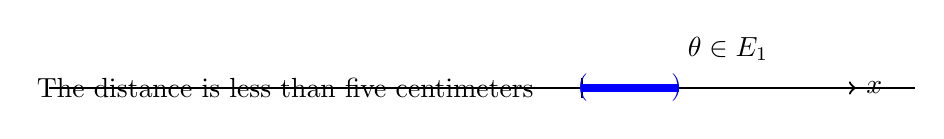
\begin{tikzpicture}[scale=0.25, thick]
				\draw[color=black] (-27, 0) to (17, 0);
				\node[align=center] at (-15, 0) {The distance is less than five centimeters};
				\node[] at (7.5, 2) {$\theta \in E_{1}$};

				\draw[|->] (0, 0) -- (14,0) node[right] {$x$};
				\draw[line width=1mm, color=blue] (0, 0) node[] {$\,($} -- (5, 0) node[] {$\!)$};
			\end{tikzpicture}
		}
		%
		\subfigure{
			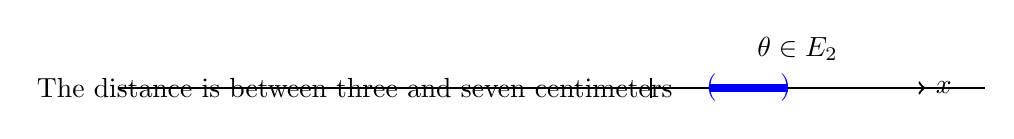
\begin{tikzpicture}[scale=0.25, thick]
				\draw[color=black] (-27, 0) to (17, 0);
				\node[align=center] at (-15, 0) {The distance is between three and seven centimeters};
				\node[] at (7.5, 2) {$\theta \in E_{2}$};

				\draw[|->] (0, 0) -- (14,0) node[right] {$x$};
				\draw[line width=1mm, color=blue] (3, 0) node[] {$\,($} -- (7,0) node[] {$\!)$};

			\end{tikzpicture}
		}
		%
		\subfigure{
			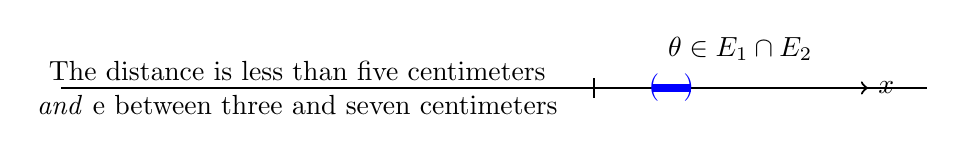
\begin{tikzpicture}[scale=0.25, thick]
				\draw[color=black] (-27, 0) to (17, 0);
				\node[align=center] at (-15, 0) {The distance is less than five centimeters \\ \textit{and} e between three and seven centimeters};
				\node[] at (7.5, 2) {$\theta \in E_{1} \cap E_{2}$};

				\draw[|->] (0, 0) -- (14,0) node[right] {$x$};
				\draw[line width=1mm, color=blue] (3, 0) node[] {$\,($} -- (5, 0) node[] {$\!)$};
			\end{tikzpicture}
		}
		%
		\subfigure{
			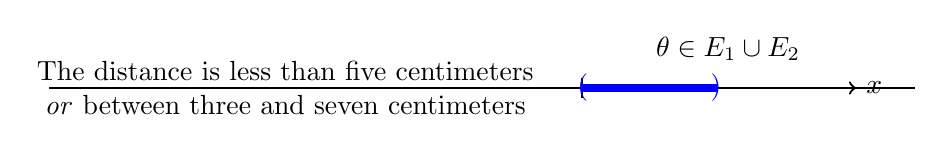
\begin{tikzpicture}[scale=0.25, thick]
				\draw[color=black] (-27, 0) to (17, 0);
				\node[align=center] at (-15, 0) {The distance is less than five centimeters \\ \textit{or} between three and seven centimeters};
				\node[] at (7.5, 2) {$\theta \in E_{1} \cup E_{2}$};

				\draw[|->] (0, 0) -- (14, 0) node[right] {$x$};
				\draw[line width=1mm, color=blue] (0, 0) node[] {$\,($} -- (7, 0) node[] {$\!)$};
			\end{tikzpicture}
		}
		%		%
		\subfigure{
			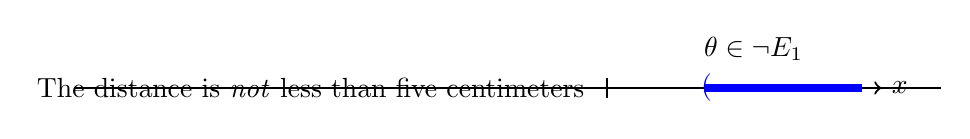
\begin{tikzpicture}[scale=0.25, thick]
				\draw[color=black] (-27, 0) to (17, 0);
				\node[align=center] at (-15, 0) {The distance is \textit{not} less than five centimeters};
				\node[] at (7.5, 2) {$\theta \in \neg E_{1}$};

				\draw[|->] (0, 0) -- (14, 0) node[right] {$x$};
				\draw[line width=1mm, color=blue] (5, 0) node[] {$\,($} -- (13, 0);
			\end{tikzpicture}
		}
	\end{figure}
\end{frame}

\begin{frame}{Discrete versus Continuous Parameters}

	Everything that has been exposed here was under the assumption that the
	parameters are discrete.
	This was done with the intent to provide an intuition what is probability.
	Not always we work with discrete parameters.
	Parameters can be continuous, such as: age, height, weight etc.
	But don't despair!
	All probability rules and axioms are valid also for continuous parameters.
	The only thing we have to do is to change all sum $\sum$ for integrals $\int$.
	For example, the third axiom of \textbf{Normalization} for \textit{continuous}
	random variables becomes:
	$$
		\int_{x \in X} p(x) dx = 1.
	$$
\end{frame}


\begin{frame}{Conditional Probability}
	\begin{defn}[Conditional Probability]
		Probability of an event occurring in case another has occurred or not. \newline \newline
		The notation we use is $P( A \mid B )$, that read as "the probability of
		observing $A$ given that we already observed $B$". \newline \newline
		$$
			\begin{aligned}
				P(A \mid B) & = \frac{\text{number of elements in$A$ e $B$}}{\text{number of elements in $B$}} \\
				P(A \mid B) & = \frac{P(A \cap B)}{(B)}
			\end{aligned}
		$$
		\newline \hspace{0.7\textwidth}
		{\footnotesize assuming that $P(B) > 0$}.
	\end{defn}
\end{frame}

\begin{frame}{Example of Conditional Probability}
	\begin{example}[Poker Texas Hold'em]
		\begin{vfilleditems}
			\item \textbf{Sample Space}: $52$ cards in a deck, $13$ types of cards and $4$ types of suits.
			\item $P(A)$: Probability of being dealt an Ace $\left( \frac{4}{52} = \frac{1}{13}\right)$
			\item $P(K)$: Probability of being dealt a King $\left( \frac{4}{52} = \frac{1}{13} \right)$
			\item $P(A \mid K)$: Probability of being dealt an Ace, given that you have already a King $\left( \frac{4}{51} \approx 0.078 \right)$
			\item $P(K \mid A)$: Probability of being dealt a King, given that you have already an Ace $\left( \frac{4}{51} \approx 0.078 \right)$
		\end{vfilleditems}
	\end{example}
\end{frame}

\begin{frame}{Caution! Not always $P(A \mid B) = P(B \mid A)$}
	In the previous example we have the symmetry $P(A \mid K) = P(K \mid A)$,
	\textbf{but not always this is true}\footnote{
		More specific, if the basal rates $P(A)$ and $P(B)$ aren't equal,
		the symmetry is broken $P(A \mid B) \neq P(B \mid A)$}
	\begin{example}[The Pope is catholic]
		\begin{vfilleditems}
			\small{
				\item $P(\text{pope})$:
				Probability of some random person being the Pope,
				something really small, 1 in 8 billion $\left( \frac{1}{8 \cdot 10^9} \right)$
				\item $P(\text{catholic})$:
				Probability of some random person being catholic,
				1.34 billion in 8 billion $\left( \frac{1.34}{8} \approx 0.17 \right)$
				\item $P(\text{catholic} \mid \text{pope})$:
				Probability of the Pope being catholic $\left( \frac{999}{1000} = 0.999 \right)$
				\item $P(\text{pope} \mid \text{catholic})$:
				Probability of a catholic person being the Pope $\left( \frac{1}{1.34 \cdot 10^9} \cdot 0.999 \approx 7.46 \cdot 10^{-10} \right)$
			}
			\item \large{\textbf{Hence}: $P(\text{catholic} \mid \text{pope}) \neq P(\text{pope} \mid \text{catholic})$}
		\end{vfilleditems}
	\end{example}
\end{frame}

\begin{frame}{A Probability Textbook Classic}
	\begin{columns}
		\begin{column}{0.6\textwidth}
			\begin{example}[Monty Hall]
				\begin{vfilleditems}
					\small
					\item A TV presenter shows you 3 doors
					\item One of them has a prize: a car!
					The others have a goat
					\item You must choose a door (that is not open or revealed)
					\item In this moment, the presenter opens one of the other two doors
					that you did not choose,
					revealing one of the two goats
					\item The presenter then asks you
					"Do you want to change your door or stay with your choice?"
				\end{vfilleditems}
			\end{example}
		\end{column}
		\begin{column}{0.4\textwidth}
			\begin{figure}
				\centering
				\def\svgwidth{\columnwidth}
				\input{../images/monty_hall.pdf_tex}
			\end{figure}
		\end{column}
	\end{columns}
\end{frame}

\begin{frame}{Solution for the Monty Hall Problem}
	\begin{idea}[Probability of winning a car]
		$$
			\begin{aligned}
				P(\text{car} \mid C_i) & = \frac{1}{3}                                                                                                                    \\
				P(\text{car})          & = \frac{1}{3} \cdot P(\text{car} \mid C_1) + \frac{1}{3} \cdot P(\text{car} \mid C_2) + \frac{1}{3} \cdot P(\text{car} \mid C_3) \\
				P(\text{car})          & = \frac{\sum^3_{i=1}P(\text{car} \mid C_i)}{3}                                                                                   \\
				P(\text{car})          & = \frac{1}{3}
			\end{aligned}
		$$
	\end{idea}
	\vfill \vfill
	$C_i$ is the event that the car is behind door $i$, $i=1,2,3$
\end{frame}

\begin{frame}[t]{Solution for the Monty Hall Problem}
	\begin{columns}[t]
		\begin{column}{0.5\textwidth}
			{\Large \textbf{Scenario 1}: Don't change doors} \newline \newline
			Simple: $$\frac{1}{3}$$
		\end{column}
		\begin{column}{0.5\textwidth}
			{\Large \textbf{Scenario 2}: Change doors} \newline \newline
			Choose any door $i$ to be $C_i = 0$
			\vfill
			$$
				\begin{aligned}
					P(\text{car}) & = 0 \cdot P(\text{car} \mid C_i) + \frac{1}{3} + \frac{1}{3} \\
					P(\text{car}) & = \frac{2}{3}
				\end{aligned}
			$$
		\end{column}
	\end{columns}
\end{frame}

\begin{frame}{Visualization of the Monty Hall Problem}
	\begin{figure}
		\centering
		\subfigure{
			
\begin{tikzpicture}[
					scale=0.55,
					header/.style = {draw, rectangle, fill = blue!50!black, minimum size = 10mm},
					level distance = 3.5cm,
					transform shape, thick,
					grow = right, sloped,
				]
				\node[header] {Your Choice}
				child{
						node[header] {Car is}
						edge from parent[draw=none]
						child{
								node[header] {Monty opens}
								edge from parent[draw=none]
								child{
										node[header] {result}
										edge from parent[draw=none]
									}
							}
					};
			\end{tikzpicture}
		}
		%
		\subfigure{
			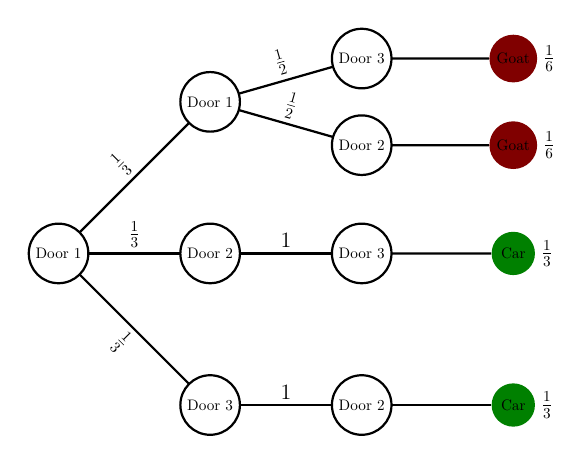
\begin{tikzpicture}[
					scale=0.55,
					door/.style = {draw, circle, minimum size = 10mm},
					car/.style = {circle, fill = green!50!black, minimum size = 10mm},
					goat/.style = {circle, fill = red!50!black, minimum size = 10mm},
					level distance = 3.5cm,
					transform shape, thick,
					grow = right, sloped,
					level 1/.style = {sibling distance=3.5cm},
					level 2/.style = {sibling distance=2cm},
					level 3/.style = {sibling distance=3cm}
				]
				\node[door] {Door 1}
				child {
				node[door] {Door 3}
				child {
				node[door] {Door 2}
				child {
				node[car, label=right:{\Large$\frac{1}{3}$}] {Car}
				}
				edge from parent
				node[above] {\Large$1$}
				}
				edge from parent
				node[below] {\Large$\frac{1}{3}$}
				}
				child {
				node[door] {Door 2}
				child {
				node[door] {Door 3}
				child {
				node[car, label=right:{\Large$\frac{1}{3}$}] {Car}
				}
				edge from parent
				node[above] {\Large$1$}
				}
				edge from parent
				node[above] {\Large$\frac{1}{3}$}
				}
				child {
				node[door] {Door 1}
				child {
				node[door] {Door 2}
				child {
				node[goat, label=right:{\Large$\frac{1}{6}$}] {Goat}
				}
				edge from parent
				node[above]  {\Large$\frac{1}{2}$}
				}
				child {
				node[door] {Door 3}
				child {
				node[goat, label=right:{\Large$\frac{1}{6}$}] {Goat}
				}
				edge from parent
				node[above]  {\Large$\frac{1}{2}$}
				}
				edge from parent
				node[above] {\Large$\frac{1}{3}$}
				};
			\end{tikzpicture}
		}
	\end{figure}
\end{frame}

\begin{frame}{Joint Probability}
	\begin{defn}[Joint Probability]
		Probability of two or more events occurring. \newline \newline
		The notation we use is $P(A, B)$, that read as
		"the probability of observing $A$ and also observing $B$". \newline \newline
		$$
			\begin{aligned}
				P(A,B) & = \text{number of elements in $A$ or $B$} \\
				P(A,B) & = P(A \cup B)                             \\
				P(A,B) & = P(B,A)
			\end{aligned}
		$$
	\end{defn}
\end{frame}

\begin{frame}{Example of Joint Probability}
	\begin{example}[Revisiting Poker Texas Hold'em]
		\begin{vfilleditems}
			{\footnotesize
				\item \textbf{Sample Space}: $52$ cards in a deck, $13$ types of cards and $4$ types of suits.
				\item $P(A)$: Probability of being dealt an Ace $\left( \frac{4}{52} = \frac{1}{13}\right)$
				\item $P(K)$: Probability of being dealt a King $\left( \frac{4}{52} = \frac{1}{13} \right)$
				\item $P(A \mid K)$: Probability of being dealt an Ace, given that you have already a King $\left( \frac{4}{51} \approx 0.078 \right)$
				\item $P(K \mid A)$: Probability of being dealt a King, given that you have already an Ace $\left( \frac{4}{51} \approx 0.078 \right)$
			}
			\item $P(A, K)$: Probability of being dealt an Ace \textit{and} being dealt a King
			$$
				\begin{aligned}
					P(A, K)                         & = P(K, A)                         \\
					P(A) \cdot P(K \mid A)          & = P(K) \cdot P(A \mid K)          \\
					\frac{1}{13} \cdot \frac{4}{51} & = \frac{1}{13} \cdot \frac{4}{51} \\
					                                & \approx 0.006
				\end{aligned}
			$$
		\end{vfilleditems}
	\end{example}
\end{frame}

%% Bivariate Normal adapted from: https://github.com/walmes/Tikz/blob/master/src/bivariate-normal.pgf
\begin{frame}{Visualization of Joint Probability versus Conditional Probability}
	\centering
	\begin{tikzpicture}[scale=0.9]
		\begin{axis}[
				domain   = -3.5:3.5,
				domain y = -3.5:3.5,
				view = {-70}{20},
				title={$P(X,Y)$ versus $P(X \mid Y=-0.75)$},
				xlabel={$X$},
				ylabel={$Y$},
				% zlabel={$SSE(\beta_0, \beta_1)$},
				zmin = -0,
				%xticklabels=\empty,
				%yticklabels=\empty,
				zticklabels=\empty,
				xtick=\empty,
				ytick={-0.75},
				ztick=\empty,
				axis z line*=none,
				axis y line*=left,
				axis x line*= bottom]
			\addplot3 [
				domain = -3.5:3.5,
				samples = 50, samples y = 0,
				thick, smooth, color = red, fill = orange, opacity = 0.75]
			(x, -0.75, {conditionalbinormal(-0.75, 0, 1, 0, 1, 0.75)});

			\draw (-3.5, -0.75, 0) -- (3.5, -0.75, 0);

			\addplot3 [
				surf,
				domain = -3.5:3.5,
				samples = 50,
				opacity = 0.15,
				faceted color = colorB,
				colormap = {blueblack}{
						color = (colorB)
						color = (colorA!50!white)
						color = (colorA)}]
			{binormal(0, 1, 0, 1, 0.7)};
		\end{axis}
	\end{tikzpicture}
\end{frame}

%% Countour plot adapted from: https://tex.stackexchange.com/a/31713/200209
\begin{frame}{Visualization of Joint Probability versus Conditional Probability}
	\begin{columns}
		\begin{column}{0.5\textwidth}
			\centering
			\begin{tikzpicture}[scale=0.5]
				\begin{axis}[
						view={0}{90},
						axis equal,
						enlarge y limits=true,
						title={$P(X,Y)$},
						xlabel={$X$},
						ylabel={$Y$},
						xtick=\empty,
						ytick={-0.75}
					]

					\draw[red, line width=2pt] (-3.5, -0.75) -- (3.5, -0.75);

					\addplot3[contour gnuplot={labels=false},domain=-3.5:3.5,domain y=-3.5:3.5]
					{exp(-( x^2 + y^2)/3 )};

				\end{axis}
			\end{tikzpicture}
		\end{column}
		\begin{column}{0.5\textwidth}
			\centering
			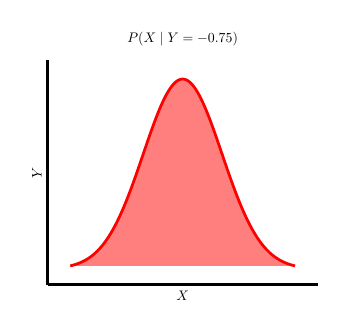
\begin{tikzpicture}[scale=0.5]
				\begin{axis}[every axis plot, line width=2pt,
						title={$P(X \mid Y=-0.75)$},
						xlabel={$X$},
						ylabel={$Y$},
						xtick=\empty,
						ytick=\empty,
						domain=-3.5:3.5,samples=200,
						axis x line*=bottom,  % no box around the plot, only x and y axis
						axis y line*=left,    % the * suppresses the arrow tips
						enlarge x limits=true % extend the axes a bit
					]

					\addplot [red, fill = red, fill opacity = 0.5] {exp(-( x^2 + -0.75^2)/3 )};
				\end{axis}
			\end{tikzpicture}
		\end{column}
	\end{columns}
\end{frame}

\subsubsection{Bayes Theorem}
\begin{frame}{Who was Thomas Bayes?}
	\begin{columns}
		\begin{column}{0.8\textwidth}
			\begin{vfilleditems}
				\item \small \textbf{Thomas Bayes} (1701 - 1761) was a statistician, philosopher
				and Presbyterian minister who is known for formulating a specific
				case of the theorem that bears his name: Bayes' theorem.
				\item \small Bayes never published what would become his most famous
				accomplishment; his notes were edited and published posthumously by
				his friend \textbf{Richard Price}.
				\item \small The theorem official name is \textbf{Bayes-Price-Laplace},
				because \textbf{Bayes} was the first to discover,
				\textbf{Price} got his notes, transcribed into mathematical notation,
				and read to the Royal Society of London,
				and \textbf{Laplace} independently rediscovered the theorem without
				having previous contact in the end of the XVIII century in France
				while using probability for statistical inference with census
				data in the Napoleonic era.
			\end{vfilleditems}
		\end{column}
		\begin{column}{0.2\textwidth}
			\centering
			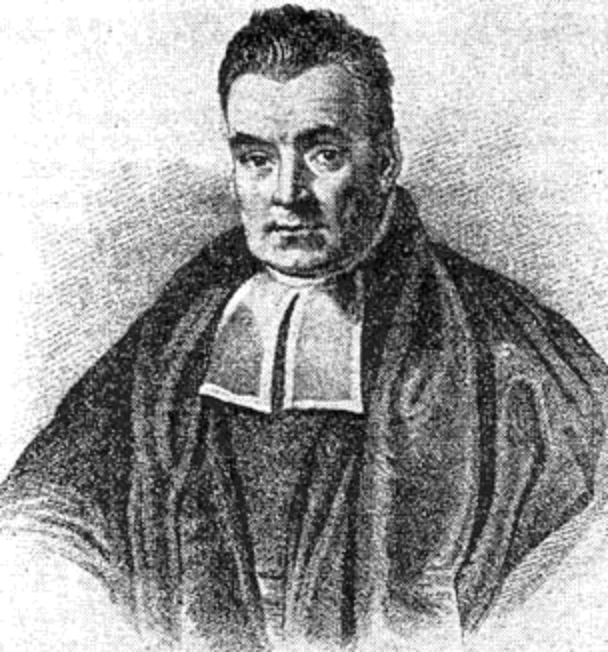
\includegraphics[width=0.9\columnwidth]{thomas_bayes.png}
		\end{column}
	\end{columns}
\end{frame}

\begin{frame}{Bayes Theorem}
	\begin{theorem}[Bayes]
		Tells us how to "invert" conditional probability: \newline \newline
		$$P(A \mid B) = \frac{P(A) \cdot P(B \mid A)}{P(B)}$$
	\end{theorem}
\end{frame}

%\begin{frame}{Prova do Teorema de Bayes}
%	Lembra que temos a seguinte identidade na probabilidade:
%	$$
%		\begin{aligned}
%			P(A,B)                 & = P(B,A)                 \\
%			P(A) \cdot P(B \mid A) & = P(B) \cdot P(A \mid B)
%		\end{aligned}
%	$$

%	Pois bem, agora passe o $P(B)$ do lado direito para o lado esquerdo dividindo:
%	$$
%		\begin{aligned}
%			P(A) \cdot P(B \mid A)              & = \overbrace{P(B)}^{\text{isso vai para $\leftarrow$}} \cdot \quad P(A \mid B) \\
%			                                    &                                                                                \\
%			\frac{P(A) \cdot P(B \mid A)}{P(B)} & = P(A \mid B)                                                                  \\
%			P(A \mid B)                         & = \frac{P(A) \cdot P(B \mid A)}{P(B)}
%		\end{aligned}
%	$$
%\end{frame}

%\begin{frame}{Mais um clássico da Probabilidade\footnote{Origem: \href{https://www.yudkowsky.net/rational/bayes}{Yudkowski - \textit{An Intuitive Explanation of Bayes’ Theorem}}}}
%	\begin{exemplo}[Cancêr de Mama]
%		\small
%		O quão acurado é o teste de \textbf{câncer de mama}?
%		\begin{vfilleditems}
%			\item \footnotesize 1\% das mulheres têm \textbf{câncer de mama} (Prevalência)
%			\item \footnotesize 80\% das mamografias detectam o \textbf{câncer de mama} (Verdadeiro Positivo)
%			\item \footnotesize 9.6\% das mamografias detectam \textbf{câncer de mama} quando não há incidência (Falso Positivo)
%		\end{vfilleditems}
%		$$
%			\begin{aligned}
%				P(C \mid +) & = \frac{P(+ \mid C) \cdot P(C)}{P(+)}                                                      \\
%				P(C \mid +) & = \frac{P(+ \mid C) \cdot P(C)}{P(+ \mid C) \cdot P(C) + P(+ \mid \neg C) \cdot P(\neg C)} \\
%				P(C \mid +) & = \frac{0.8 \cdot 0.01}{0.8 \cdot 0.01 + 0.096 \cdot 0.99}                                 \\
%				P(C \mid +) & \approx 0.0776
%			\end{aligned}
%		$$
%	\end{exemplo}
%\end{frame}


%\begin{frame}{Porquê o teorema de Bayes é Importante?}
%	\begin{idea}[Podemos Inverter a Probabilidade Condicional]
%		$$
%			\begin{aligned}
%				P(\text{hipótese} \mid \text{dados}) = \frac{P(\text{hipótese}) \cdot P(\text{dados} \mid \text{hipótese})}{P(\text{data})}
%			\end{aligned}
%		$$
%	\end{idea}
%	Mas isso não é o $p$-valor? \textcolor{red}{\textbf{NÃO!}}
%\end{frame}

%\subsection{Estatística Frequentista versus Bayesiana}
%\subsubsection{O que são $p$-valores e Intervalos de Confiança}
%\begin{frame}{O que é o $p$-valor?}
%	\begin{defn}[$p$-valor]
%		$p$-valor é a probabilidade de obter resultados no mínimo tão
%		extremos quanto os que foram observados, dado que a hipótese nula
%		$H_0$ é verdadeira
%		$$P(D \mid H_0)$$
%	\end{defn}
%\end{frame}

%\begin{frame}{O que \textbf{não é} o $p$-valor!}
%	\centering
%	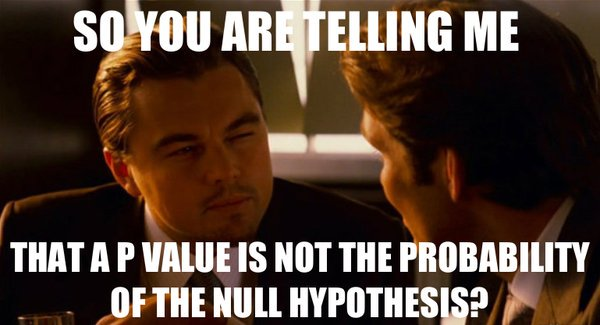
\includegraphics[width=0.7\textwidth]{meme-pvalue.jpg}
%\end{frame}

%\begin{frame}{O que \textbf{não é} o $p$-valor!}
%	\begin{vfilleditems}
%		\item \textbf{$p$-valor não é a probabilidade da Hipótese nula}
%		- Famosa confusão entre $P(D \mid H_0)$ e $P(H_0 \mid D)$.
%		Para obter a $P(H_0 \mid D)$ você precisa de estatística Bayesiana.
%		\item \textbf{$p$-valor não é a probabilidade dos dados serem produzidos pelo acaso}
%		- \textcolor{red}{Não!} Ninguém falou nada de acaso.
%		\item \textbf{$p$-valor mensura o tamanho do efeito de um teste estatístico}
%		- Também \textcolor{red}{não}... $p$-valor não diz nada sobre o tamanho do efeito.
%		Apenas sobre se o quanto os dados observados divergem do esperado sob a hipótese nula.
%		Além disso, $p$-valores podem ser "hackeados" de diversas maneiras \parencite{head2015extent}.
%	\end{vfilleditems}
%\end{frame}

%\begin{frame}{A relação entre $p$-valor e $H_0$}
%	Para descobrir o $p$-valor, \textbf{descubra a $H_0$ que está por trás dele}.
%	Sua definição nunca mudará, pois ela sempre é $P(D \mid H_0)$:
%	\begin{vfilleditems}
%		\item \textbf{Teste $t$}: $P(D \mid \text{a diferença entre os grupos é zero})$
%		\item \textbf{ANOVA}: $P(D \mid \text{não há diferença entre os grupos})$
%		\item \textbf{Regressão}: $P(D \mid \text{coeficiente é nulo})$
%		\item \textbf{Shapiro-Wilk}: $P(D \mid \text{população é distribuída como uma normal})$
%	\end{vfilleditems}
%\end{frame}

%\begin{frame}{O que são Intervalos de Confiança?}
%	\begin{columns}
%		\begin{column}{0.8\textwidth}
%			\begin{defn}[Intervalos de Confiança]
%				\begin{quotation}
%					Um intervalo de confiança de X\% para um parâmetro é um intervalo
%					$(a, b)$ gerado por um procedimento que em amostragem repetida
%					tem uma probabilidade de X\% de conter o valor verdadeiro do
%					parâmetro, para todos os valores possíveis do parâmetro
%				\end{quotation}
%				\vfill \vfill
%				\textcite{neyman1937outline} (o "pai" dos intervalos de confiança)
%			\end{defn}
%		\end{column}
%		\begin{column}{0.2\textwidth}
%			\centering
%			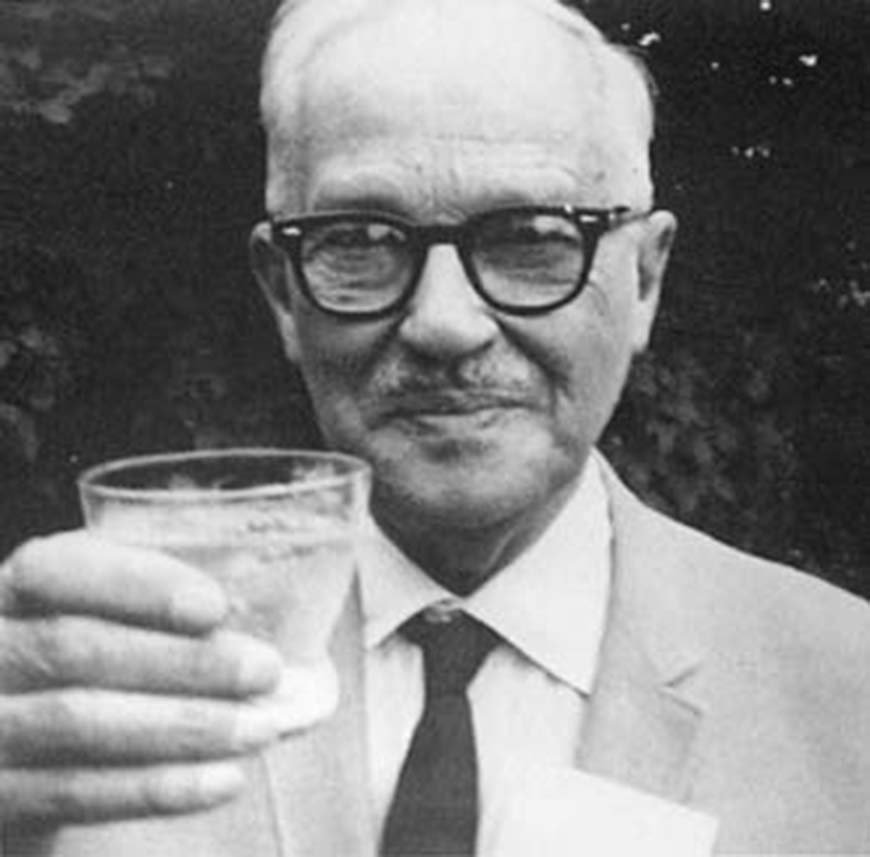
\includegraphics[width=0.9\columnwidth]{neyman.jpeg}
%		\end{column}
%	\end{columns}
%\end{frame}

%\begin{frame}{O que são Intervalos de Confiança?}
%	\begin{exemplo}[Intervalo de Confiança de uma Política Pública]
%		Digamos que você executou uma análise estatística para comparar
%		eficácia de uma política pública em dois grupos e você obteve a
%		diferença entre a média desses grupos. Você pode expressar essa
%		diferença como um intervalo de confiança. Geralmente escolhemos a
%		confiança de 95\%. Isso quer dizer que \textbf{95 estudos de 100},
%		que usem o \textbf{mesmo tamanho de amostra e população-alvo},
%		aplicando o \textbf{mesmo teste estatístico}, esperarão encontrar
%		um resultado de diferenças de média entre grupos entre o intervalo
%		de confiança.
%	\end{exemplo}
%	\footnotesize \textcolor{red}{Não diz nada sobre a sua \textbf{população-alvo},
%		mas sim sobre a sua \textbf{amostra} num processo maluco de \textbf{amostragem infinita}...}
%\end{frame}

%\begin{frame}{Intevalos de Confiança versus Intervalos da Posterior}
%	\centering
%	\begin{tikzpicture}
%		\begin{axis}[every axis plot, line width=2pt,
%				xmin=0, xmax=4,
%				ymin=0, ymax=1.5,
%				ylabel=\empty,
%				xlabel={$\theta$},
%				samples=200,
%				axis x line*=bottom, % no box around the plot, only x and y axis
%				axis y line*=left,
%				enlarge x limits=true,
%			] % extend the axes a bit

%			\addplot [blue, domain=0:4, forget plot] {lognormal(0, 2)};
%			\addplot+ [
%				mark=none,
%				area legend,
%				line width=0pt,
%				color=blue,
%				fill=blue, fill opacity=0.5,
%				domain=0.25950495026507125:3.8534910373715427
%			]
%			{lognormal(0, 2)} \closedcycle;
%			\addlegendentry{50\% Posterior}
%			\addplot[red, mark=none] (-0.09, 1.4739034450607542) to (0.09, 1.4739034450607542);
%			\addlegendentry{MLE}
%			\draw [red] (0,0) to (0, 1.4739034450607542);
%		\end{axis}
%	\end{tikzpicture}
%\end{frame}

%\begin{frame}{Intevalos de Confiança versus Intervalos da Posterior}
%	\centering
%	\begin{tikzpicture}
%		\begin{axis}[every axis plot, line width=2pt,
%				xmin=-3, xmax=14,
%				%ymin=0, ymax=1.5,
%				ylabel=\empty,
%				xlabel={$\theta$},
%				samples=200,
%				axis x line*=bottom, % no box around the plot, only x and y axis
%				axis y line*=left,
%				enlarge x limits=true,
%				%legend pos=outer north east, %there is one default value for the `legend pos' that is outside the axis
%				%legend cell align=left, % so the legend looks a bit better
%			] % extend the axes a bit

%			\addplot [blue, domain=-3:14, forget plot] {sumtwonormals(2, 1, 0.6, 10, 1, 0.4)};
%			\addplot+ [
%				mark=none,
%				area legend,
%				line width=0pt,
%				color=blue,
%				fill=blue, fill opacity=0.5,
%				domain=1.8:9.7
%			]
%			{sumtwonormals(2, 1, 0.6, 10, 1, 0.4)} \closedcycle;
%			\addlegendentry{50\% Posterior}
%			\addplot[red, mark=none] (1.5, 0.24) to (2.5, 0.24);
%			\addlegendentry{MLE}
%			\draw [red] (2,0) to (2, 0.24);
%		\end{axis}
%	\end{tikzpicture}
%\end{frame}

%\begin{frame}{Mas por quê eu nunca vejo estatística sem $p$-valor?}
%	\begin{columns}
%		\begin{column}{0.8\textwidth}
%			Não tem como entendermos $p$-valores se não compreendermos as suas
%			origens e trajetória histórica. A primeira menção do termo foi feita
%			pelo estatístico Ronald Fisher em 1925 \parencite{fisher1925statistical}:
%			\begin{quotation}
%				[$p$-valor é] índice que mede a força da evidência contra a hipótese nula
%			\end{quotation}
%			\begin{vfilleditems}
%				\item Para quantificar a força da evidência contra a hipótese nula, Fisher defendeu
%				"$p<0.05$ como um nível padrão para concluir que há evidência contra a hipótese testada"
%				\item "Não seremos frequentemente perdidos se traçarmos uma linha convencional de 0.05"
%			\end{vfilleditems}
%		\end{column}
%		\begin{column}{0.2\textwidth}
%			\centering
%			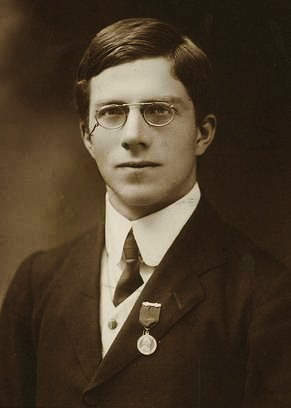
\includegraphics[width=0.9\columnwidth]{fisher.jpg}
%		\end{column}
%	\end{columns}
%\end{frame}

%\begin{frame}{$p = 0.06$}
%	\begin{vfilleditems}
%		\item Como o $p$-valor é uma probabilidade, ele é uma quantidade contínua.
%		\item Não há razão para diferenciarmos um $p$ de 0.049 contra um $p$ de 0.051.
%		\item Robert Rosenthal, um psicólogo já dizia "Deus ama $p$ de 0.06 tanto quanto um $p$ de 0.05"~\parencite{rosnow1989statistical}.
%	\end{vfilleditems}
%\end{frame}

%\begin{frame}{Mas por quê eu nunca ouvi falar de Estatística Bayesiana?\footnote{\textit{inverse probability} é como o teorema de Bayes era chamado no começo do século XX}}
%	\begin{columns}
%		\begin{column}{0.8\textwidth}
%			\begin{quotation}
%				… it will be sufficient … to reaffirm my personal conviction …
%				that the theory of inverse probability is founded upon an error,
%				and must be wholly rejected.
%			\end{quotation}
%			\vfill \vfill
%			\textcite{fisher1925statistical}
%		\end{column}
%		\begin{column}{0.2\textwidth}
%			\centering
%			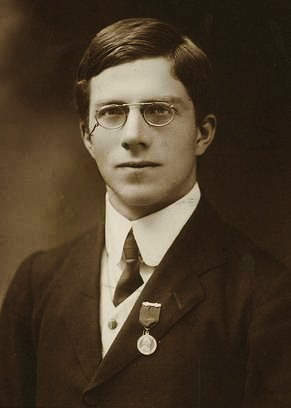
\includegraphics[width=0.9\columnwidth]{fisher.jpg}
%		\end{column}
%	\end{columns}
%\end{frame}

%\begin{frame}{Dentro de todo não Bayesiano há um Bayesiano querendo sair\footnote{Dennis Lindley "Inside every nonBayesian there is a Bayesian struggling to get out"}}
%	\begin{columns}
%		\begin{column}{0.8\textwidth}
%			\begin{vfilleditems}
%				\item No último ano de sua vida, Fisher publicou um artigo \parencite{fisherExamplesBayesMethod1962} examinando as possibilidades dos métodos Bayesianos, mas com as probabilidades a \textit{priori} a serem determinadas experimentalmente.
%				\item Inclusive alguns autores especulam \parencite{jaynesProbabilityTheoryLogic2003} que se Fisher estivesse vivo hoje, ele provavelmente seria um "Bayesiano".
%			\end{vfilleditems}
%		\end{column}
%		\begin{column}{0.2\textwidth}
%			\centering
%			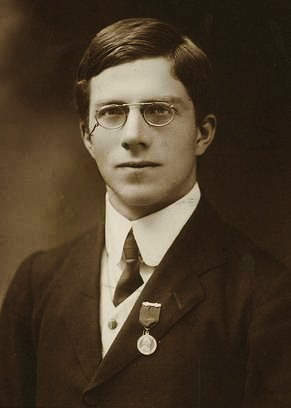
\includegraphics[width=0.9\columnwidth]{fisher.jpg}
%		\end{column}
%	\end{columns}
%\end{frame}

%\subsection{Estatística Bayesiana}
%\begin{frame}{Teorema de Bayes como Motor de Inferência}
%	\footnotesize Agora que você já sabe o que é probabilidade e o que é o teorema de Bayes, vou propor o seguinte modelo:
%	$$
%		\underbrace{P(\theta \mid y)}_{\text{Posterior}} = \frac{\overbrace{P(y \mid  \theta)}^{\text{Verossimilhança}} \cdot \overbrace{P(\theta)}^{\textit{Priori}}}{\underbrace{P(y)}_{\text{Constante Normalizadora}}}
%	$$
%	\begin{vfilleditems}
%		\item \footnotesize $\theta$ -- parâmetro(s) de interesse
%		\item \footnotesize $y$ -- dados observados
%		\item \footnotesize \textbf{\textit{Priori}}: probabilidade prévia do valor do(s) parâmetro(s)
%		\item \footnotesize \textbf{Verossimilhança}: probabilidade dos dados observados condicionados aos valores do(s) parâmetro(s)
%		\item \footnotesize \textbf{Posterior}: probabilidade posterior do valor do(s) parâmetros após observamos os dados $y$
%		\item \footnotesize \textbf{Constante Normalizadora}: $P(y)$ não faz sentido intuitivo. Essa probabilidade é transformada e pode ser interepretada como algo que existe apenas para que o resultado de $P(y \mid \theta) P(\theta)$ seja algo entre 0 e 1 -- uma probabilidade válida.
%	\end{vfilleditems}
%\end{frame}

%\begin{frame}{Teorema de Bayes como Motor de Inferência}
%	A estatísica Bayesiana nos permite \textbf{quantificar diretamente a incerteza}
%	relacionada ao valor de um ou mais parâmetros do nosso modelo condicionado aos
%	dados observados. Isso é a \textbf{característica principal} da estatística
%	Bayesiana. Pois estamos estimando diretamente $P(\theta \mid y)$ por meio do
%	teorema de Bayes. A estimativa resultante é totalmente intuitiva:
%	simplesmente quantifica a intercerteza que temos sobre o valor de um ou mais
%	parâmetro condicionado nos dados, nos pressupostos do nosso modelo
%	(verossimilhança) e na probabilidade prévia que temos sobre tais valores.
%\end{frame}

%\subsubsection{Vantagens da Estatísca Bayesiana}
%\begin{frame}{Estatística Bayesiana vs Frequentista}
%	%\begin{table}[h!]
%	\small
%	\begin{tabular}{|l|p{.3\textwidth}|p{.3\textwidth}|}
%		\toprule
%		                       & \textcolor{blue}{\textbf{Estatística Bayesiana}} & \textcolor{red}{\textbf{Estatística Frequentista}}                  \\ \midrule
%		\textbf{Dados}         & Fixos –- Não Aleatórios                          & Incertos –- Aleatórios                                              \\ \midrule
%		\textbf{Parâmetros}    & Incertos –- Aleatórios                           & Fixos –- Não Aleatórios                                             \\ \midrule
%		\textbf{Inferência}    & Incerteza sobre o valor do parâmetro             & Incerteza sobre um processo de amostragem de uma população infinita \\ \midrule
%		\textbf{Probabilidade} & Subjetiva                                        & Objetiva (mas com diversos pressupostos dos modelos)                \\ \midrule
%		\textbf{Incerteza}     & Intervalo de Credibilidade –- $P(\theta \mid y)$ & Intervalo de Confiança –- $P(y \mid \theta)$                        \\
%		\bottomrule
%	\end{tabular}
%	%\end{table}
%\end{frame}

%\begin{frame}{Vantagens da Estatística Bayesiana}
%	\begin{vfilleditems}
%		\item Abordagem Natural para expressar Incerteza
%		\item Habilidade de incorporar Informações Prévias
%		\item Maior Flexibilidade do Modelo
%		\item Distribuição Posterior completa dos Parâmetros
%		\item Propagação Natural da Incerteza
%	\end{vfilleditems}
%	\small \textbf{Principal Desvantagem}: Velocidade lenta de estimativa de modelos\footnote{\textit{e.g.} 30 segundos ao invés de 3 segundos na abordagem frequentista}
%\end{frame}

%\begin{frame}{O começo do fim da Estatística Frequentista}
%	\begin{vfilleditems}
%		\small
%		\item Saiba que você está em um momento da história no qual a Estatística está passando por grandes mudanças
%		\item Acredito que a estatística frequentista, em especial a maneira que qualificamos evidências e hipóteses
%		com $p$-valores se transformará de maneira "significante".
%		\item Há cinco anos atrás, a \textit{American Statistical Association} (ASA) publicou uma declaração sobre
%		$p$-valores \parencite{Wasserstein2016}. A declaração diz exatamente o que falamos aqui: Os conceitos principais do teste de significância de hipótese nula e, em particular $p$-valores não conseguem prover o que os pesquisadores requerem deles. Apesar do que dizem muitos livros de estatística, materiais de ensinos e artigos publicados, $p$-valores abaixo de 0,05 não "provam" a realidade de nada. Nem, chegando a esse ponto, os $p$-valores acima de 0,05 refutam alguma coisa.
%		\item A declaração da ASA tem mais de 3.600 citações provocando impacto relevante.
%	\end{vfilleditems}
%\end{frame}

%\begin{frame}{O começo do fim da Estatística Frequentista}
%	\begin{vfilleditems}
%		\small
%		\item Um simpósio internacional foi promovido em 2017 que originou uma edição especial de acesso aberto da
%		\textit{The American Statistician} dedicada à maneiras práticas de abandonarmos $p < 0.05$
%		\parencite{wassersteinMovingWorld052019}.
%		\item Logo na sequência vieram mais tentativas e reivindicações.
%		Em setembro de 2017, a \textit{Nature Human Behaviour} publicou um editorial propondo que o nível de
%		significância do $p$-valor seja reduzido de $0.05$ para $0.005$ \parencite{benjaminRedefineStatisticalSignificance2018}
%		Diversos autores, inclusive muitos estatísticos altamente influentes e importantes argumentaram que esse simples passo
%		ajudaria a combater o problema da crise de replicabilidade da ciência, que muitos acreditam ser a principal
%		consequência do uso abusivo de $p$-valores \parencite{Ioannidis2019}.
%		\item Além disso, muitos foram um passo além e sugerem que a ciência descarte de uma vez por todas $p$-valores
%		\parencite{ItTimeTalk2019,lakensJustifyYourAlpha2018}. Muitos sugerem (eu inclusive) que a principal ferramenta
%		de inferência seja a estatística Bayesiana \parencite{amrheinScientistsRiseStatistical2019, Goodman1180, vandeschootBayesianStatisticsModelling2021}
%	\end{vfilleditems}
%\end{frame}
